%\documentclass[conference]{IEEEtran}
\documentclass[journal,onecolumn,12pt]{IEEEtran}

\usepackage{graphicx}
\usepackage{bm}% bold math

\usepackage{epsfig}

%\usepackage{cite}
%\usepackage[bookmarks=true,pdfstartview=FitH]{hyperref}
\usepackage[bookmarks=true,pdfstartview=FitH,,bookmarksopen=true,colorlinks,citecolor=blue,filecolor=green,linkcolor=blue,urlcolor=blue]{hyperref}
\usepackage{bookmark}
\usepackage[cmex10]{amsmath}
\usepackage{algpseudocode}
\usepackage{algorithm}
\usepackage{array}
\usepackage[caption=false]{subfig}
%\usepackage{fixltx2e}
\usepackage{stfloats}
\usepackage{url}
\usepackage{multirow}
\usepackage{threeparttable}

% correct bad hyphenation here
\hyphenation{op-tical net-works semi-conduc-tor}

\begin{document}

\title{Energy-efficient and Cross-layer Networking in Mobile MIMO-OFDM Systems}

\author{\IEEEauthorblockN{Yongsen MA} \\
\IEEEauthorblockA{Shanghai Jiao Tong University \\
E-mail: mayongsen@gmail.com}
}

% make the title area
\maketitle
%
%\begin{abstract}
%%\boldmath
%The abstract goes here.
%\end{abstract}


\section{Statement of Purpose}

The wireless networks have experienced rapid development in recent years, which leads to the increase of traffic loads and users requirements. The wide expansion of wireless services has brought serious challenges to the issues of spectrum efficiency and required data rate. Recently, WLANs (Wireless Local Area Networks) based on 802.11n have enjoyed tremendous growth due to the ever-increased demands of high-bandwidth applications. Moreover, with the increasing popularity of smartphones, the growth of mobile 802.11n is expected to continue unabated \cite{Bala2010wifi}. On the other hand, the power consumption of wireless communications is becoming increasingly vital to a more efficient and longer lasting mobile battery in mobile wireless systems. The continued success of mobile 802.11n depends on their ability to efficiently configure different PHY/MAC enhancements based on MIMO-OFDM technology, and here comes the question of \textbf{how to get energy-efficient trade-off between reliability and data rate in mobile MIMO-OFDM systems?}

In order to solve this problem, some approaches on energy-efficient rate adaption have been carried out based on simulations \cite{5510775} \cite{6214414} or experiments \cite{Peng:2011:TPS:2030613.2030628} \cite{Li:2012:ERA:2348543.2348585}. Although these works present different solutions such as optimization, packet delivery probing and channel state prediction, they are all based on the information of channel state and link quality. So a basic consideration is the \textit{accurate channel state estimation and link quality measurement with relatively lower overhead}. This is challenging in that multi-configuration in mobile 802.11n not only requires far more samples to acquire sufficient information for all possible channel settings, but also introduces significant complications in channel modeling. Furthermore, channels are more vulnerable to environmental variability and terminal mobility in mobile 802.11n. Therefore, accurate channel measurement and prediction is becoming increasingly important in mobile 802.11n networks.

The measurement-based Packet Delivery Ratio and Received Signal Strength (PDR-RSS) model is widely used for performance analysis in static wireless networks \cite{reis2006model}. It has been successfully exploited in 802.11a/b/g for upper layer applications such as capacity analysis \cite{kashyap2007capacity} and spectrum allocation \cite{k.rayanchu:fluid:}. However, PDR-RSS model exhibits a large transition window in wireless channels due given the fact that the frequency selectivity of the wideband 802.11 channel is not captured by RSS. Halperin \textit{et al.} \cite{Halperin2010predictable} proposed predictable model to determine the subcarrier Signal to Noise Ratio (SNR) using Channel State Information (CSI) and then aggregate into a global metric called eSNR, which provided better characterization for link quality. But CSI-based measurement in 802.11n can dramatically increase the complexity of channel estimation and modeling. It requires \textit{O}$(k\cdot m \cdot n)$ measures to obtain the complete CSI matrix for $m \times n$ MIMO with $k$ subcarriers ($k=56/114$ for 20/40MHz channels) \cite{CSI-SF}. Furthermore, commonly used 802.11n wireless devices only provide CSI reports for unicast packets, which clearly affect the efficiency of collecting CSI matrices. Hence, the tradeoff exists between measurement overhead and accuracy which is worthy to be explored, especially in mobile environments.

Prior works on the PDR-RSS modeling are mostly static \cite{kashyap2007capacity} \cite{kolar2011mesh} \cite{reis2006model}. Moreover, a single measurement metric, either packet-level (PDR) or physical-level (RSS), is utilized by upper layer applications\cite{judd2008efficient} \cite{zhang2008practical}. The PDR-RSS model can overcome the channel quality capturing problem if PDR and RSS are jointly considered. This is further supported by exploiting the multi-configuration properties in 802.11n, in which the transition window exhibits diversity distribution for different configurations from our extensive experiments. It indicates that there exists certain configuration(s) for current RSS that can ensure PDR being out of transition windows. This key observation motivates us developing an on-line PDR-RSS modeling framework, which utilizes real-time PDR and RSS to update PDR-RSS model dynamically and configure PHY/MAC settings in mobile 802.11n.
%
%\subsection{Traffic Requirements}
%\begin{figure}
%\centering
%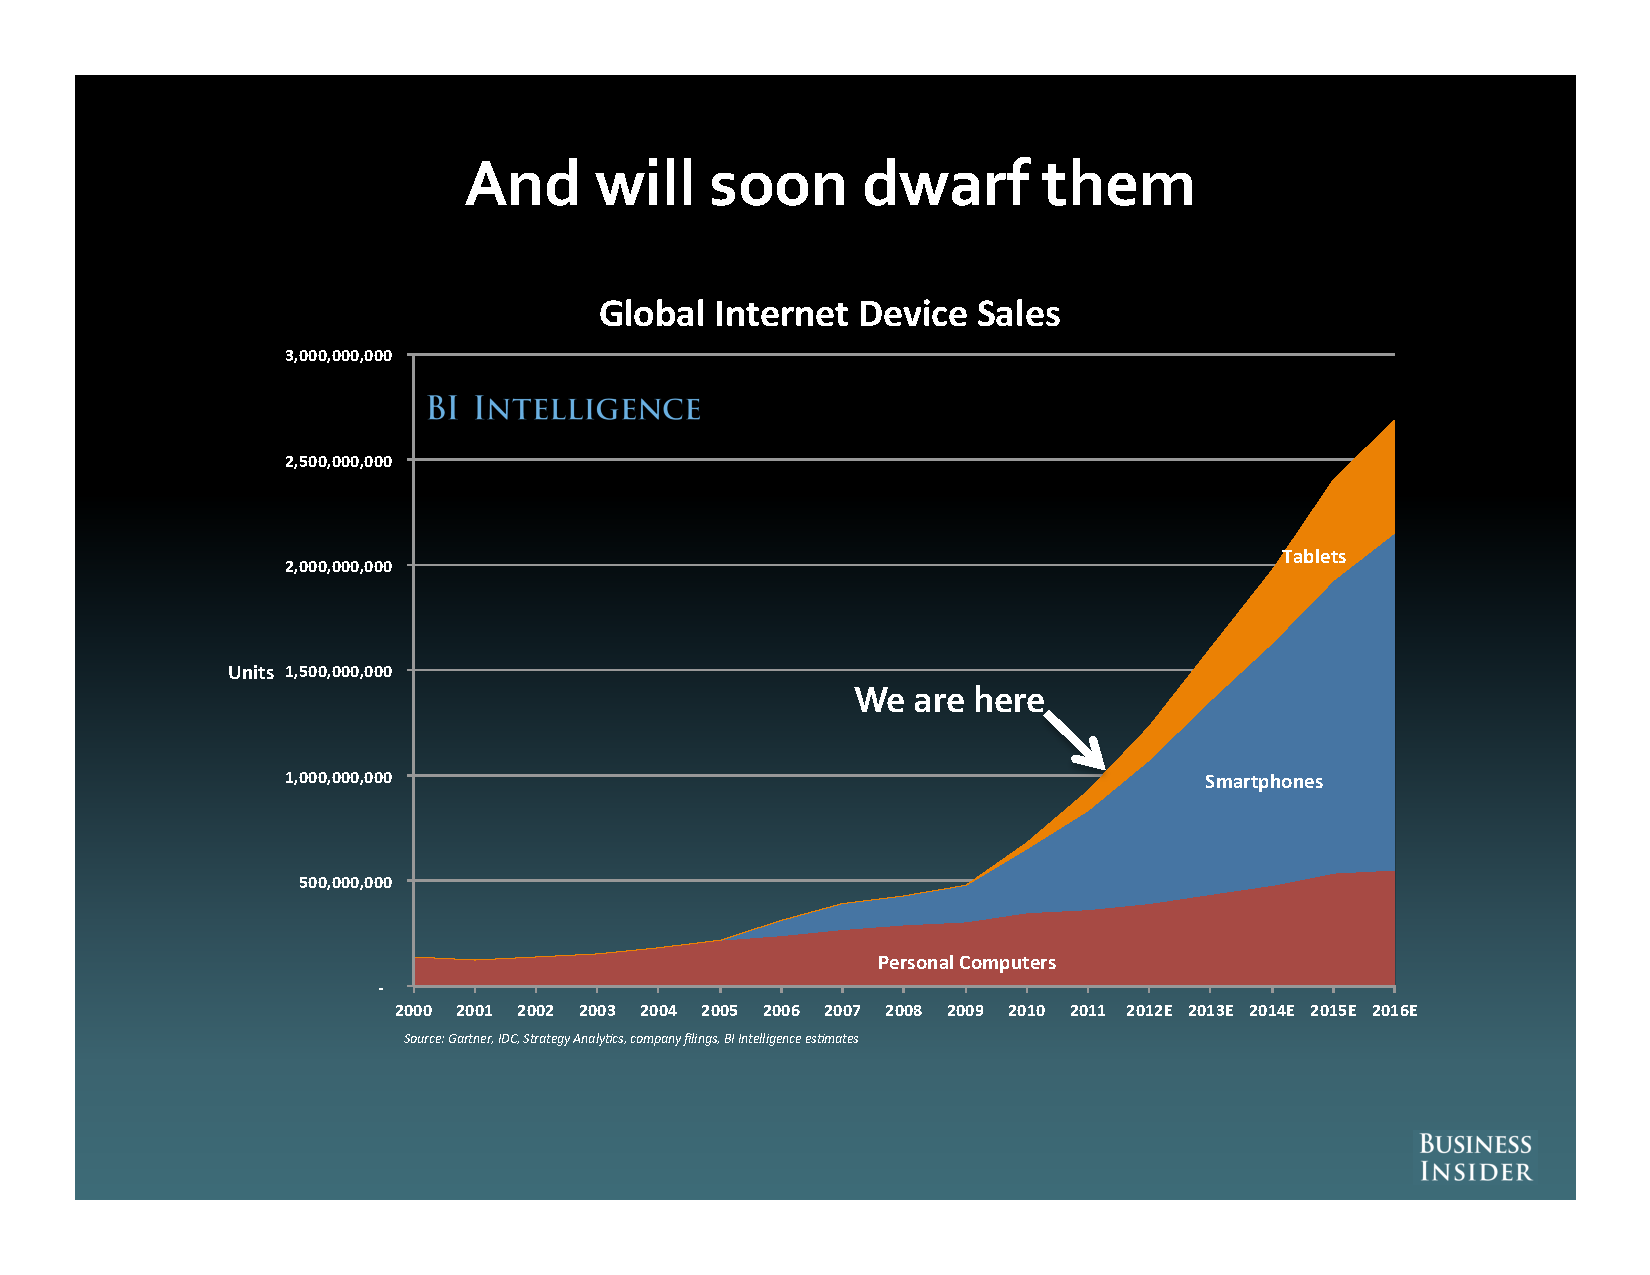
\includegraphics[width=0.8\textwidth]{device_trend.pdf}
%\caption{Global Internet Device Sales.}
%\label{fig:device_trend}
%\end{figure}
%
%\begin{figure}
%\centering
%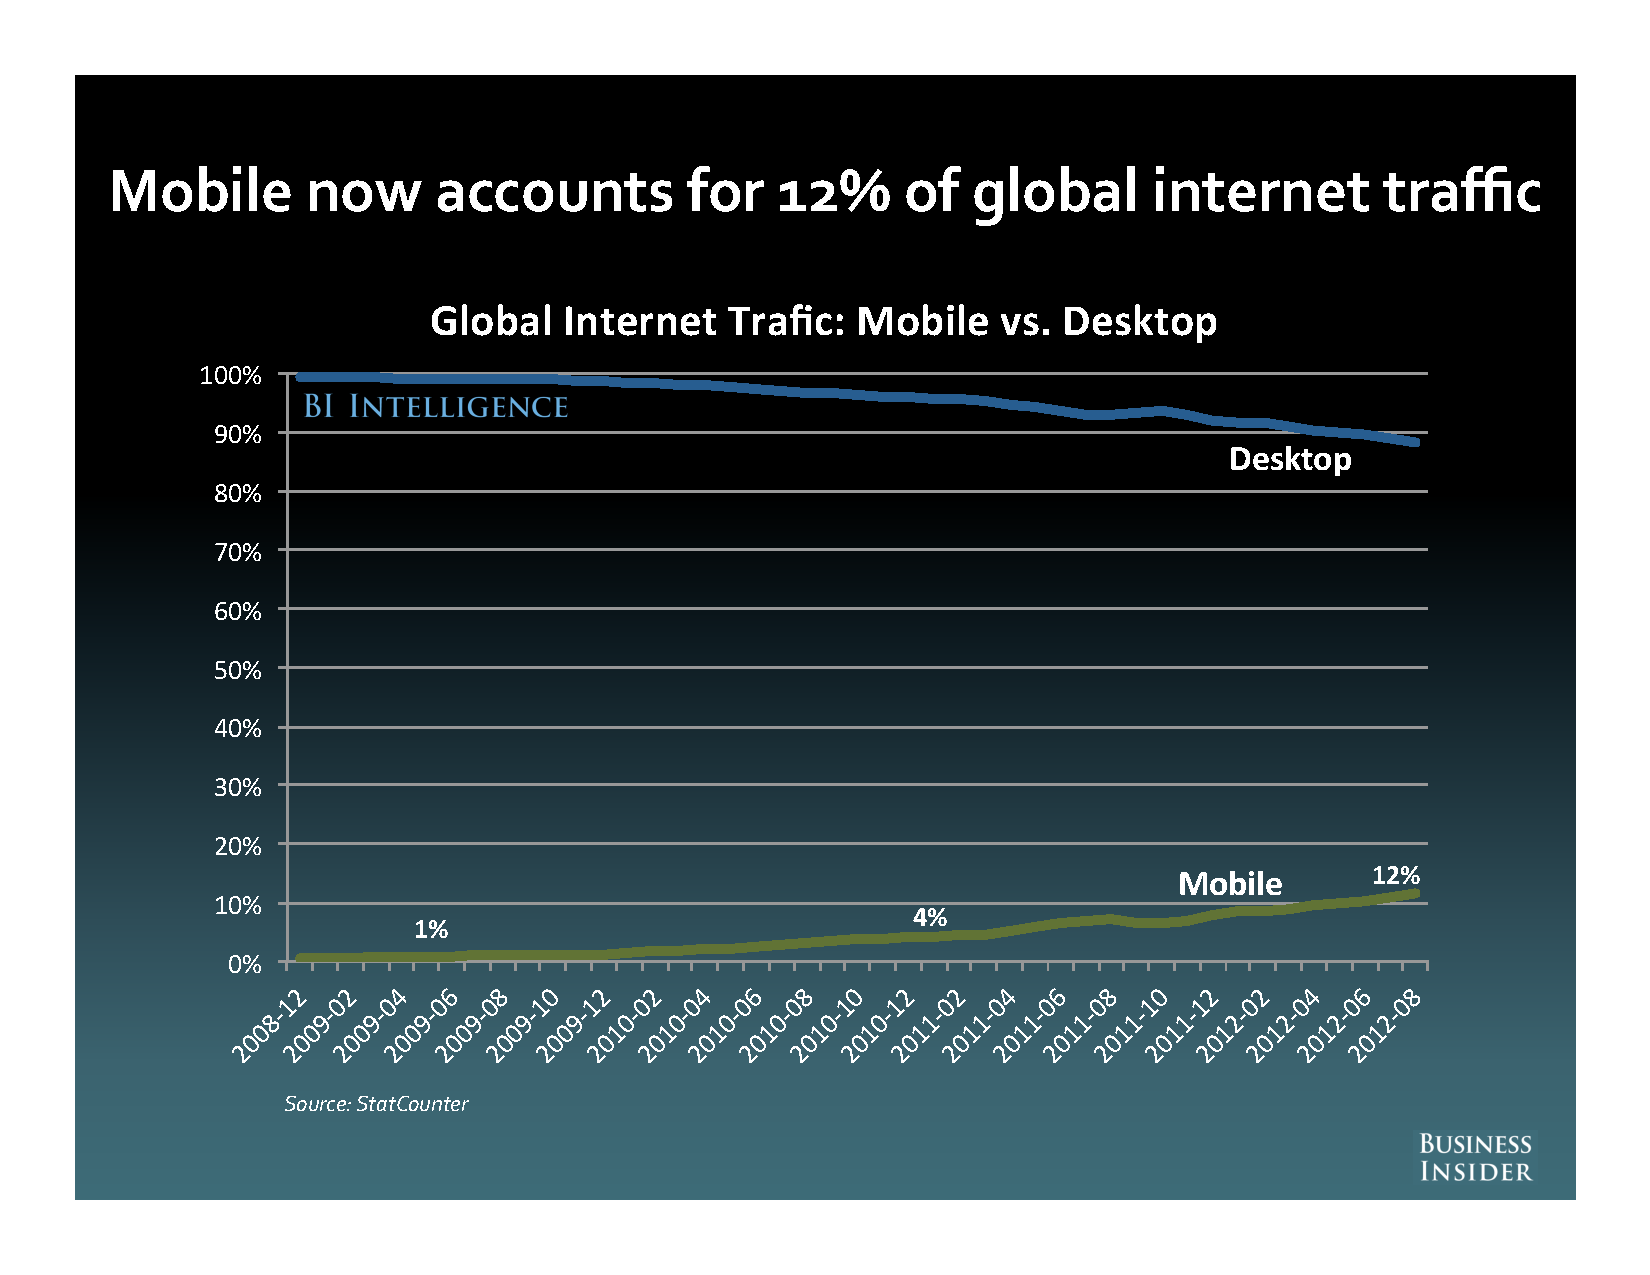
\includegraphics[width=0.8\textwidth]{mobile_desktop.pdf}
%\caption{Global Internet Traffic: Mobile vs. Desktop.}
%\label{fig:mobile_desktop}
%\end{figure}
%
%\begin{figure}
%\centering
%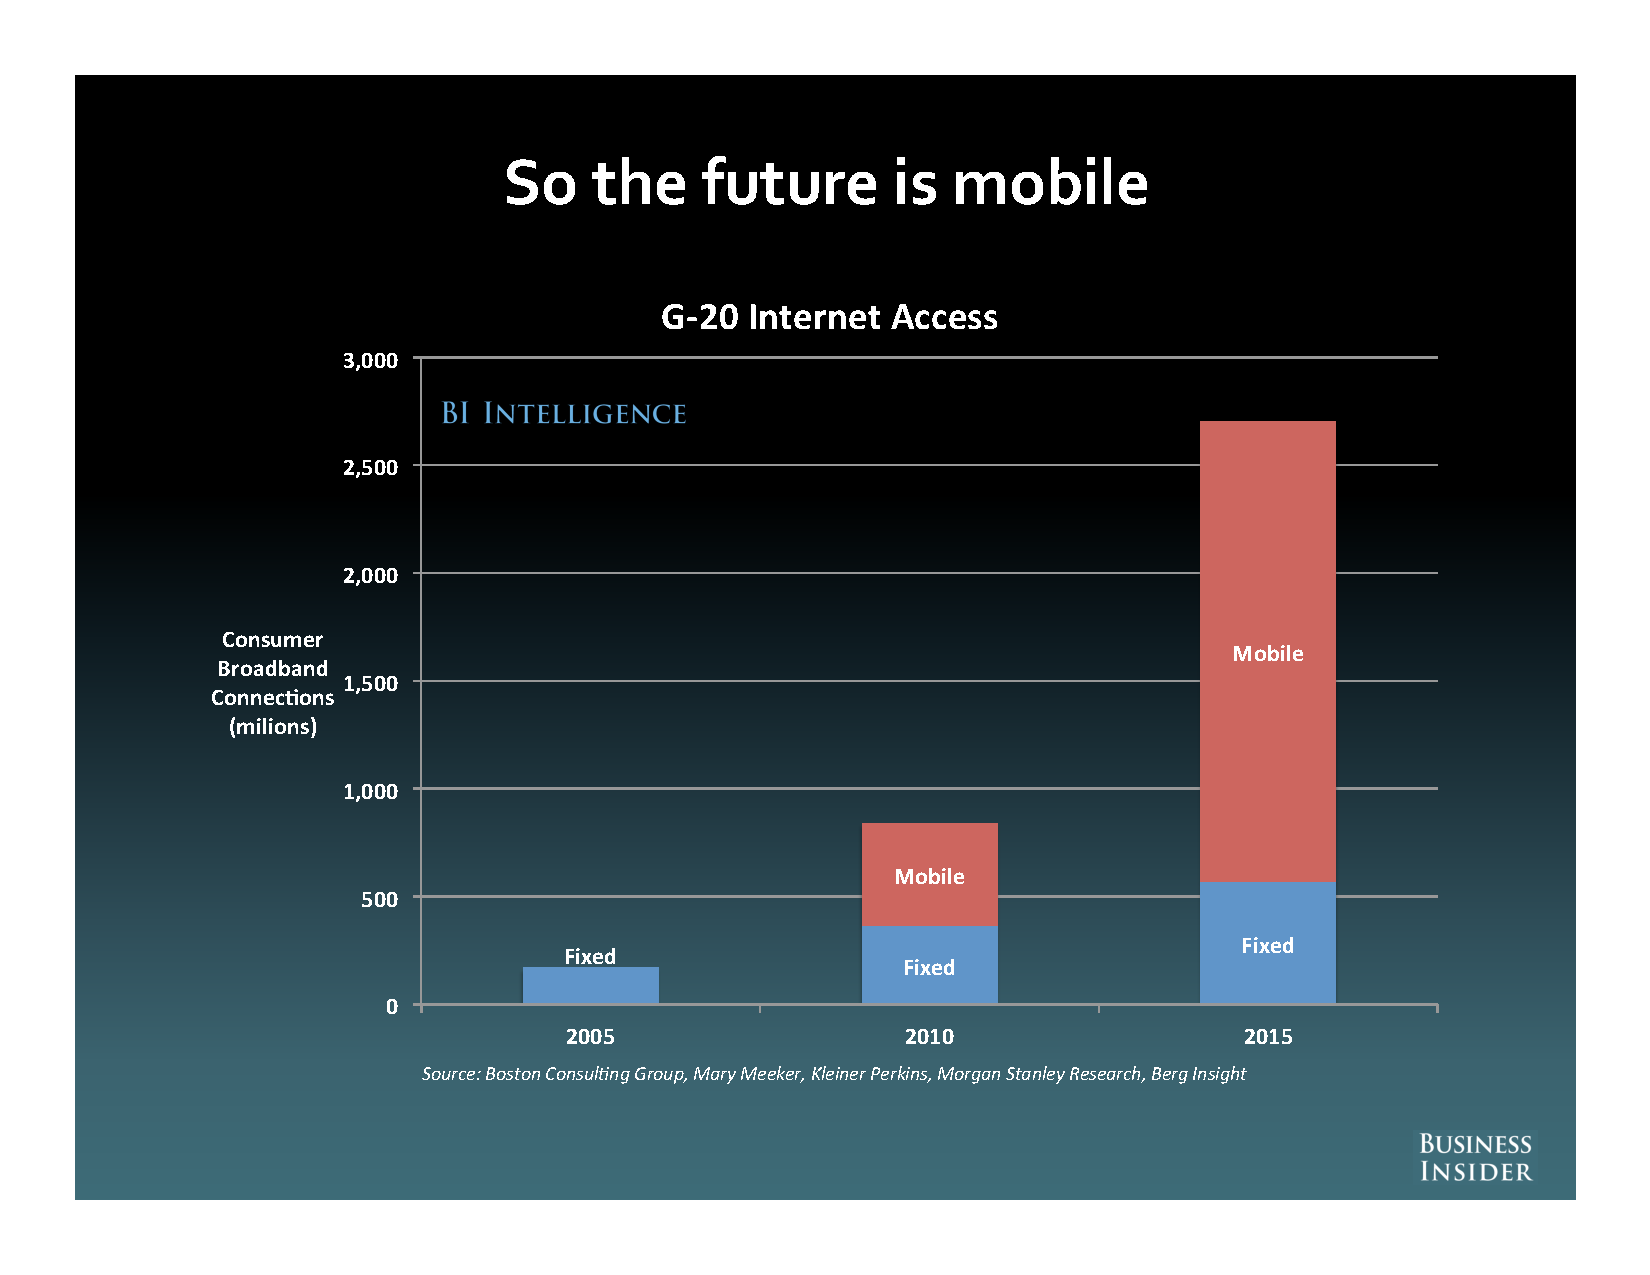
\includegraphics[width=0.8\textwidth]{mobile_trend.pdf}
%\caption{Internet Access: Mobile vs. Fixed.}
%\label{fig:mobile_trend}
%\end{figure}
%
%\begin{figure}
%\centering
%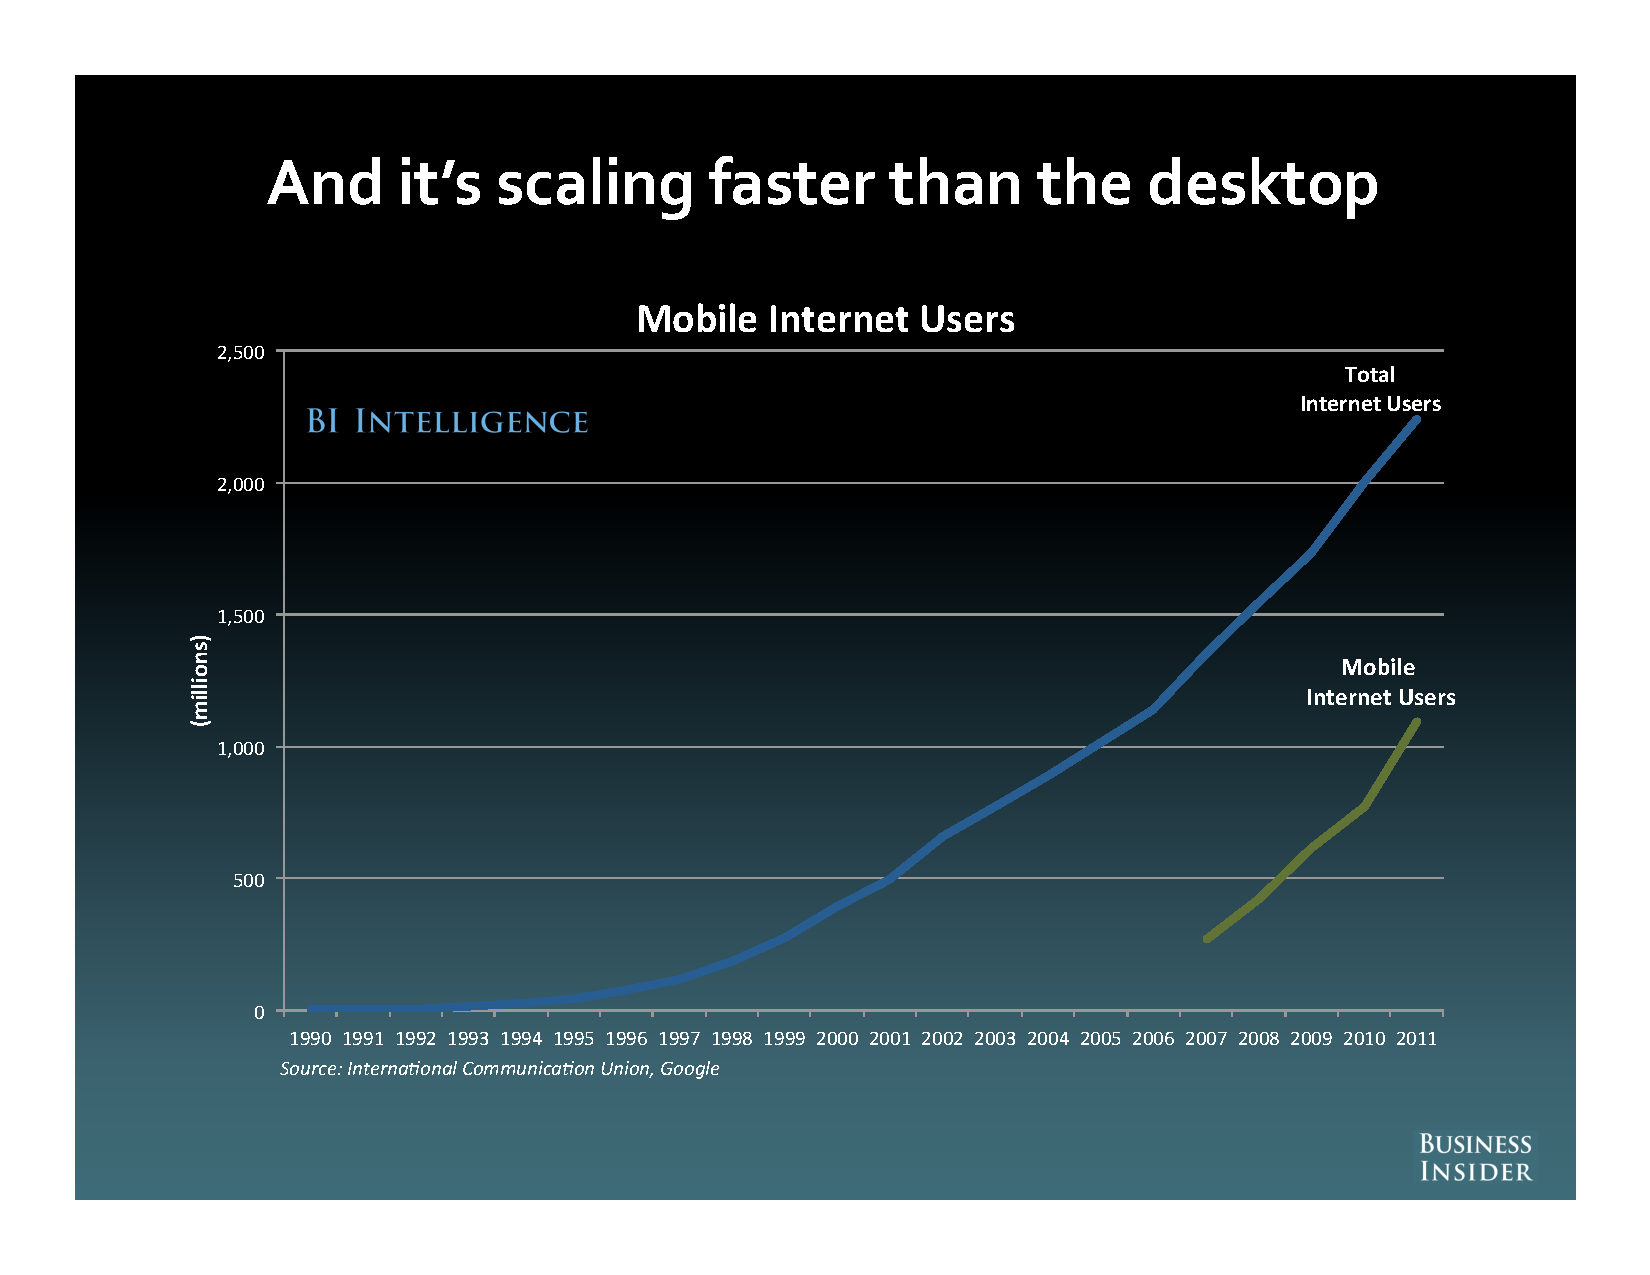
\includegraphics[width=0.8\textwidth]{mobile_users.pdf}
%\caption{Mobile Internet Users.}
%\label{fig:mobile_users}
%\end{figure}
%
%\subsection{Spectrum Efficiency}
%
%\subsection{Energy Efficiency}

\section{Research Questions}

We use our testbeds to experimentally identify the deficiencies of related work on channel measurement and prediction methods. The goal is to describe the motivation of on-line PDR-RSS modeling framework and critical issues in the new design. To illustrate our findings, we first present a general framework for current channel measurement and prediction methods based on PDR and PDR-RSS model, which is shown in Fig.~\ref{offlinemodel}. The main features in this framework are as follows: (1) static EWMA measure for PDR; (2) static data set and PDR-RSS model; (3) single measurement metric (PDR or RSS) input.
\begin{figure}[!t]
\centerline{
    \subfloat[Time varying]{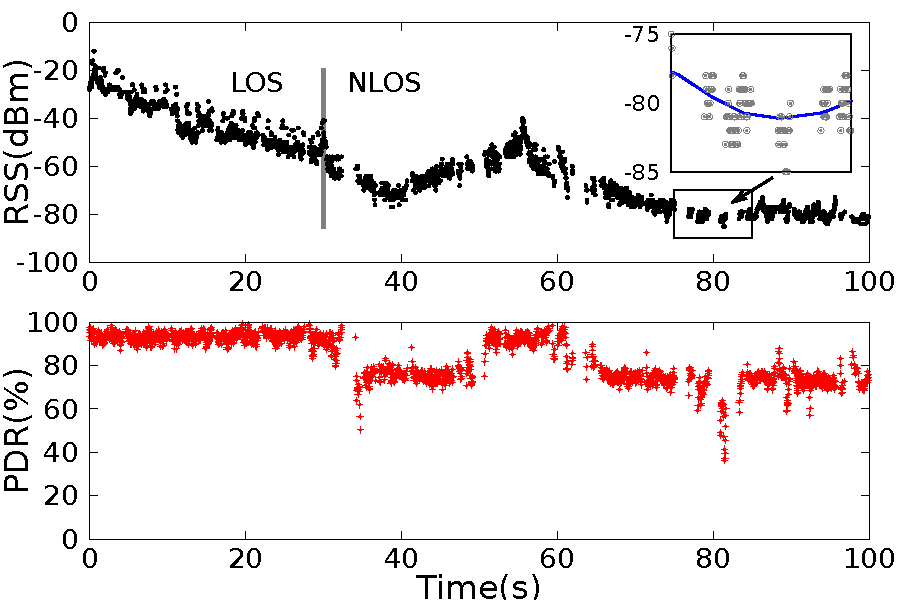
\includegraphics[width=0.4\textwidth]{time.pdf}
    \label{time_vary}
}
    \subfloat[Location difference]{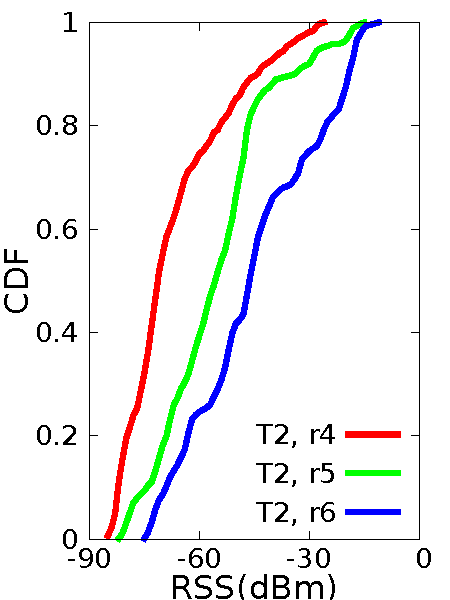
\includegraphics[width=0.2\textwidth]{cdfrss.pdf}
    \label{cdf_rss}
}
    \subfloat[PDR-RSS model]{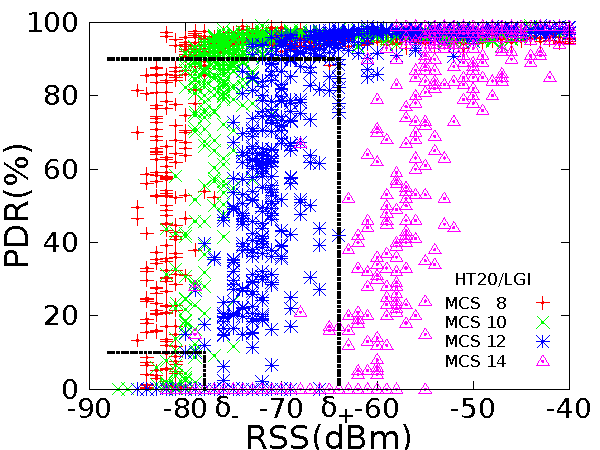
\includegraphics[width=0.36\textwidth]{pdr.pdf}
    \label{cdf_rss}
}
}
\caption{Characteristics of PDR and RSS in mobile 802.11n, composed of both of LOS and NLOS scenarios.}
\label{time}
\end{figure}

\textbf{PDR Measure Accuracy.} Static EWMA is widely used in PDR measure \cite{ath9k} \cite{minstrel} \cite{wong2008wireless}, whose update time interval is set fixed to 50ms or 100ms. However, dynamic PDR would reduce the measure accuracy of EWMA, especially when operating at high data rates. The following experiments show that PDR is vulnerable to spatial and temporal diversity in mobile 802.11n networks. RSS and PDR measurements were conducted along different routes by Atheros's 2T2R 802.11n model AR9382 at 5GHz band. Fig.~\ref{time_vary} illustrates that both RSS and PDR encounter with sudden decline in short time scale. The Cumulative Distribution Functions (CDF) of RSS measures with the same 802.11n cards along route r4 to r6 are given in Fig.~\ref{cdf_rss}, which illustrates the spatial diversity feature of network status. Fig.~\ref{pdr_over} shows a specific measurement example for data rate of 78Mbps measured by the same way in Fig.~\ref{time_vary}, where EWMA will overestimate 20\% of PDR when there is a sudden decline. Thus, it is expected to develop dynamic PDR measurement method to increase the accuracy in mobile environments. Prior works on rate adaption in mobile environments are only concerned with RSS measurement \cite{chen2011ram} \cite{judd2008efficient}. To the best of our knowledge, there has been no examination on the measurement and prediction for PDR in fast changing channels.
\begin{figure}[!t]
\centerline{
    \subfloat[PDR overestimation]{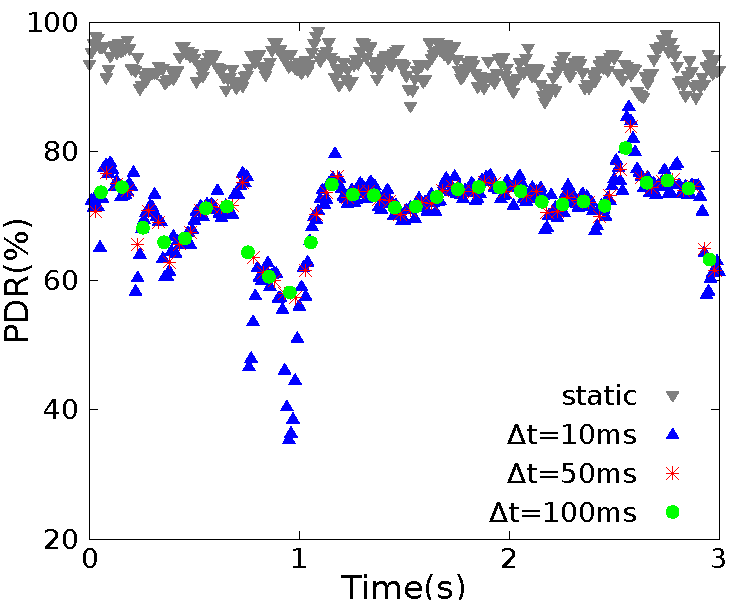
\includegraphics[width=0.45\textwidth]{pdrvary.pdf}
    \label{pdr_over}
}
    \subfloat[MCS selection]{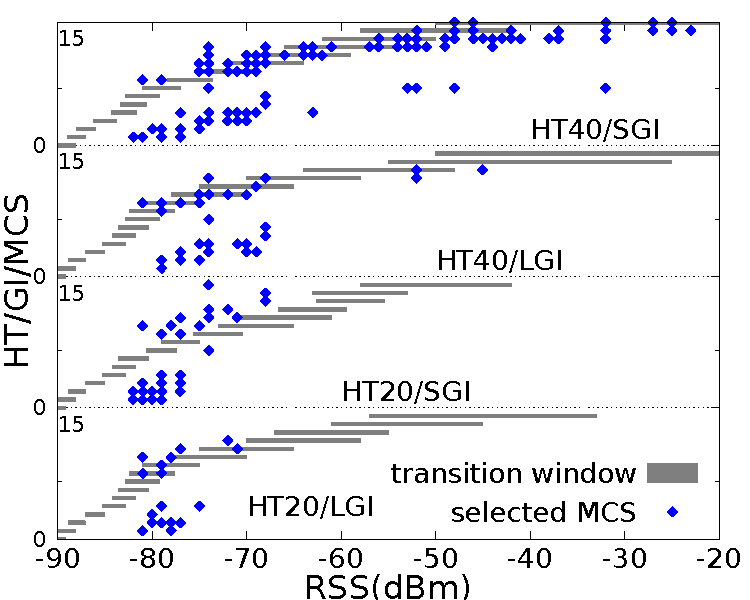
\includegraphics[width=0.45\textwidth]{MCS.pdf}
    \label{MCS}
}
}
\caption{(a) EWMA with update periods of 50/100ms will overestimate 20\% of PDR when there is a sudden decline; (b) Large parts of selected HT/GI/MCS fall within the transition window, especially for high data rates.}
\label{pdr-rss}
\end{figure}
\begin{figure}[!t]
\centering
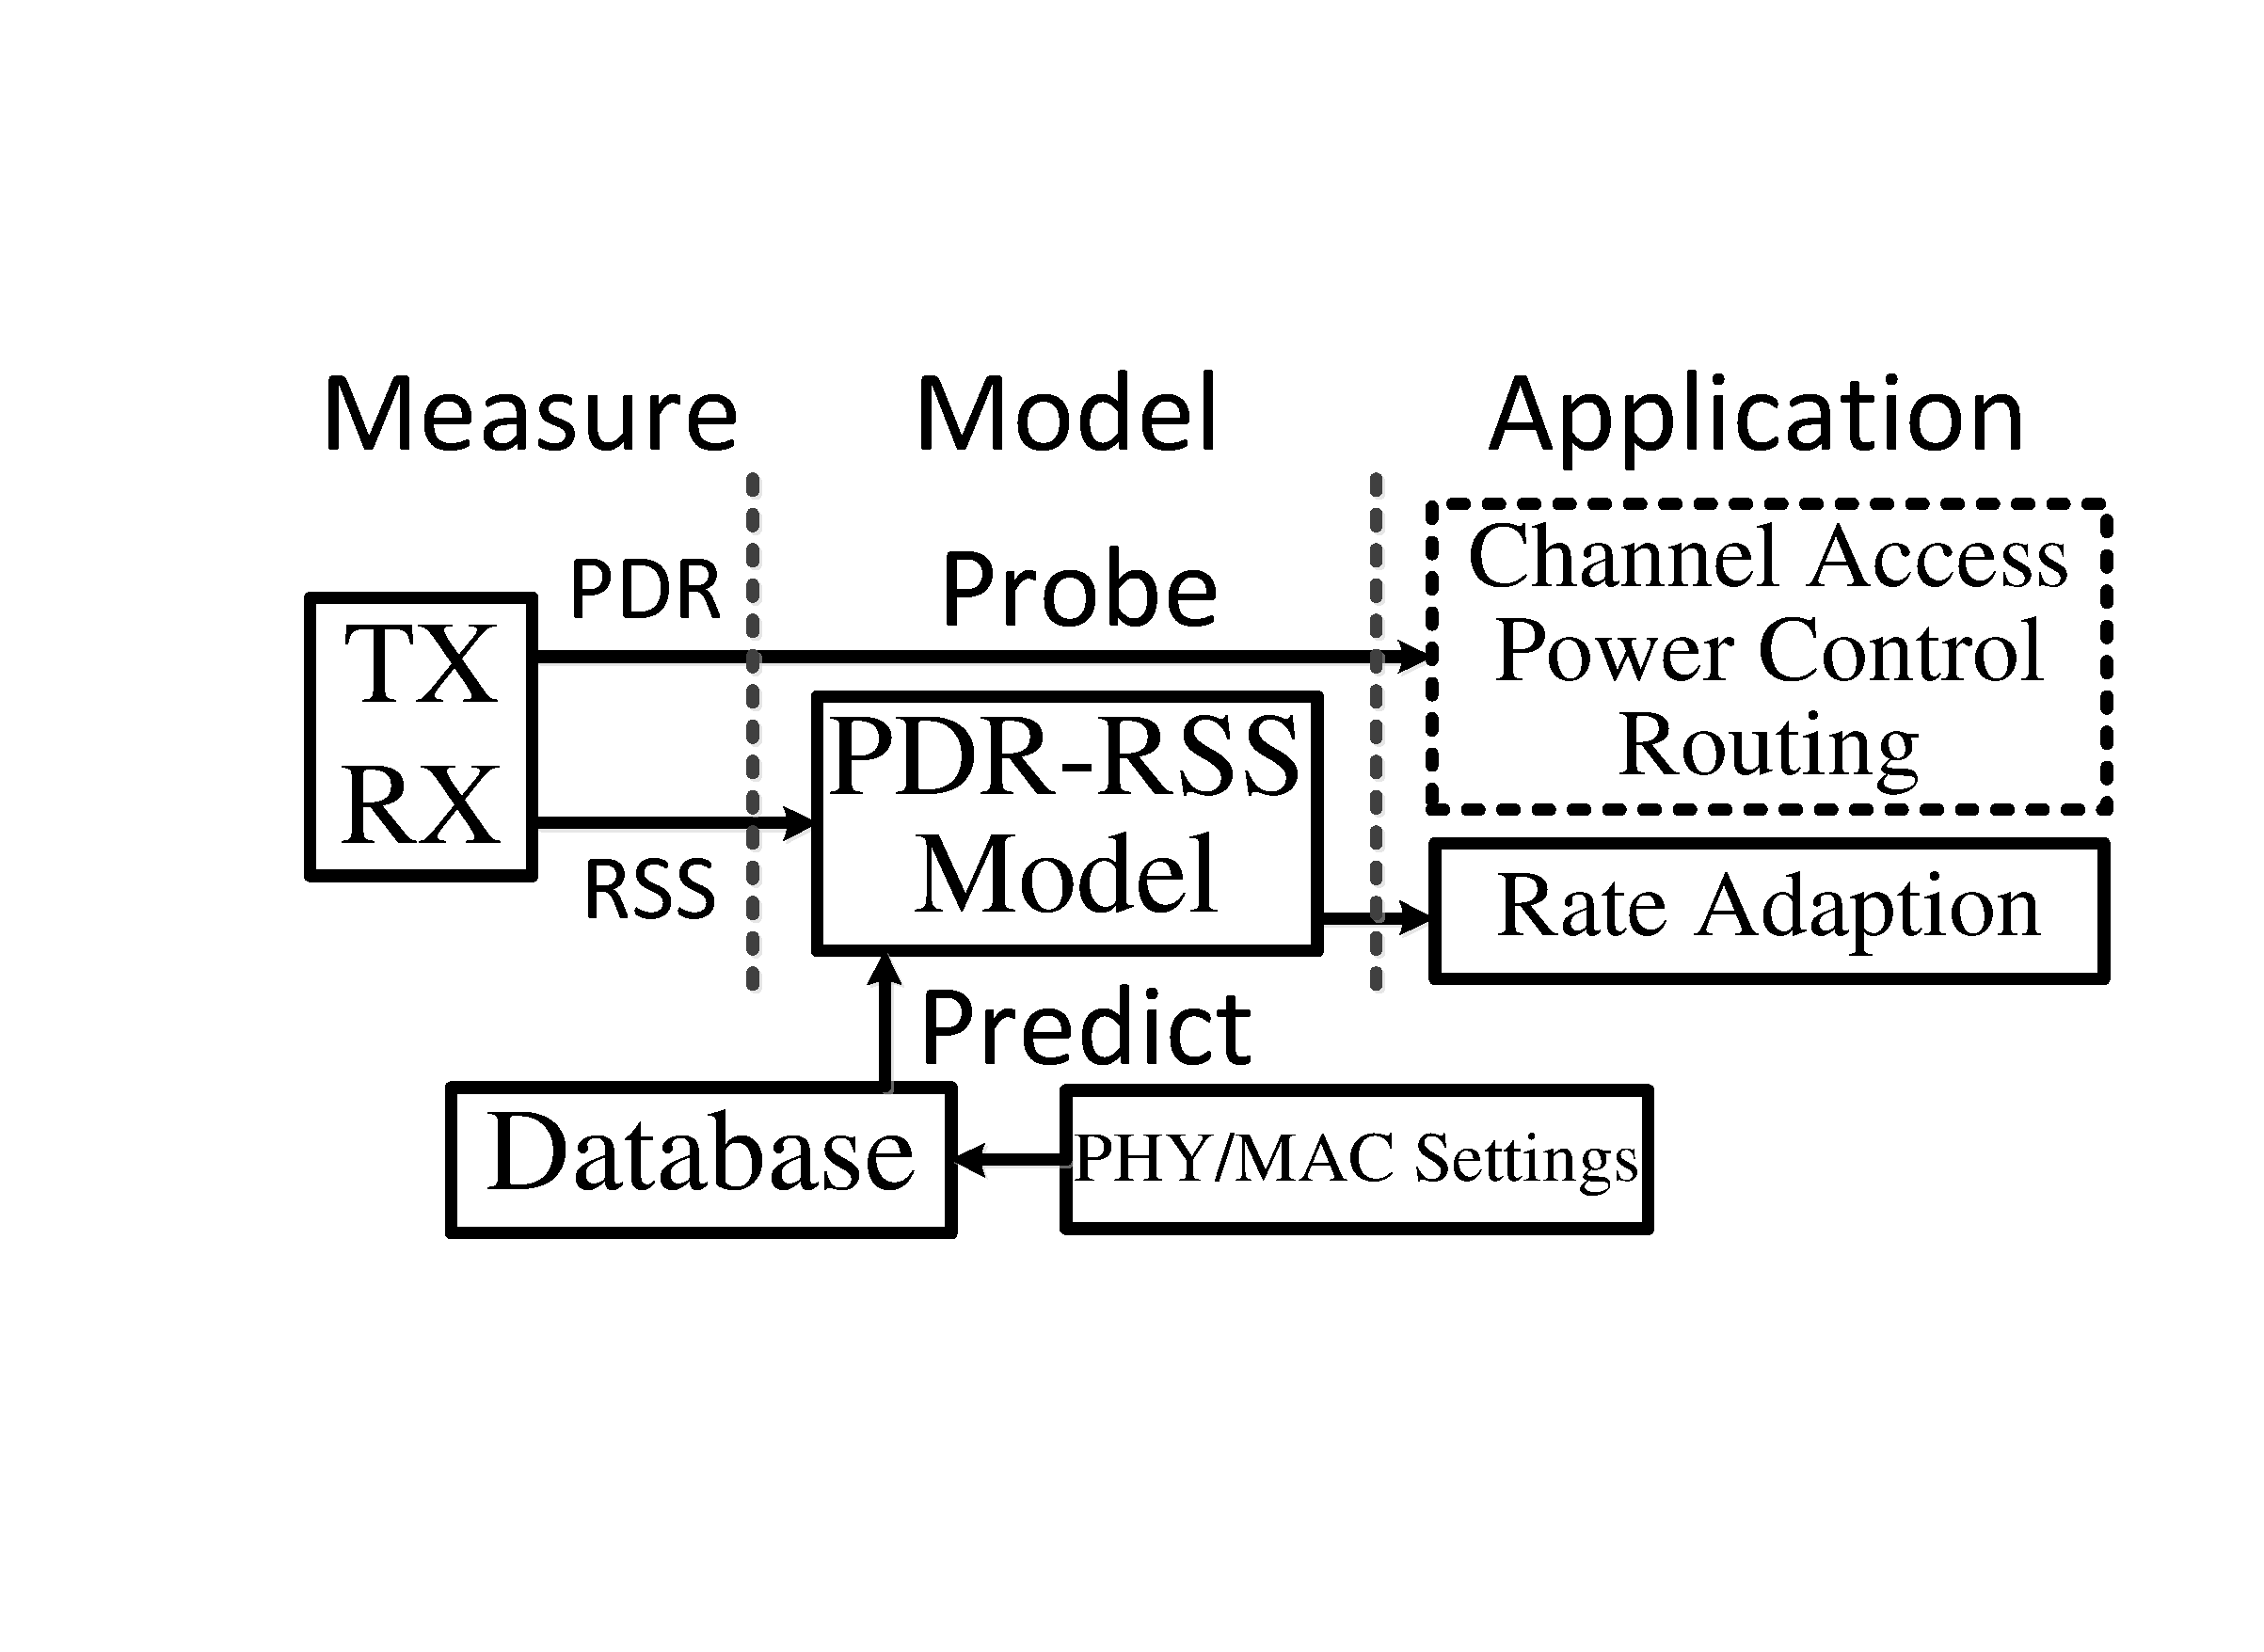
\includegraphics[width=0.45\textwidth]{modeling1.pdf}
\caption{General static PDR-RSS modeling framework.}
\label{offlinemodel}
\end{figure}

\textbf{Transition Windows.} Since 802.11n standard incorporates several enhancements including channel bonding, spatial multiplexing, frame aggregation and SGI, it is a basic problem that how to switch between different operating configurations for better suiting the radio environments. The complexity stems from the large transition window of PDR-RSS model in 802.11n \cite{Halperin2010predictable}. This situation will be worse when PDR is overestimated by static measurement approach in fast changing channels. Fig.~\ref{MCS} gives an example of rate selection results which is carried out along route r5. The gray lines, which are generated by on-line PDR-RSS modeling, are the transition windows for each individual HT/GI/MCS selection. For every four parts separated by HT/GI options, the selected MCS falling on the right of transition region means it can get high PDR under this setting. There are about 34\% falling into the transition window, and even 8\% are worse that locating on the left of the transition window. However, the good news is that the transition windows exhibit diversity distribution for different MCS selection and channel assignment from Fig.~\ref{MCS}. This indicates that there exists certain configuration(s) for current RSS that can ensure PDR being out of transition window. It provides a hint that we can configure different PHY/MAC enhancements at the right of gray line by jointly utilizing the real-time PDR and RSS, which improves the network throughput with high reliability.

To sum up, 802.11n PHY/MAC enhancements make the PDR measurement and online modeling more complicated, and mobile wireless connections are highly changing. These factors significantly reduce the prediction accuracy and rate selection efficiency in mobile 802.11n networks. The key is to design an online PDR-RSS model to address the following issues: (1) high-accuracy PDR measurement; (2) dynamic PDR-RSS model update; (3) efficient configuration(s) output. The on-line PDR-RSS modeling framework needs to address three critical issues:
\begin{enumerate}
  \item \textit{How to accurately measure PDR with low overhead in fast changing channels?}
  \item \textit{How to characterize the relationship among PDR, RSS and 802.11n multi-configuration?}
  \item \textit{How to update the characterized relationship on-line and derive the set of configurations with certain reliable performance guaranteeing at current PDR and RSS?}
\end{enumerate}

\begin{figure}[!t]
\centering
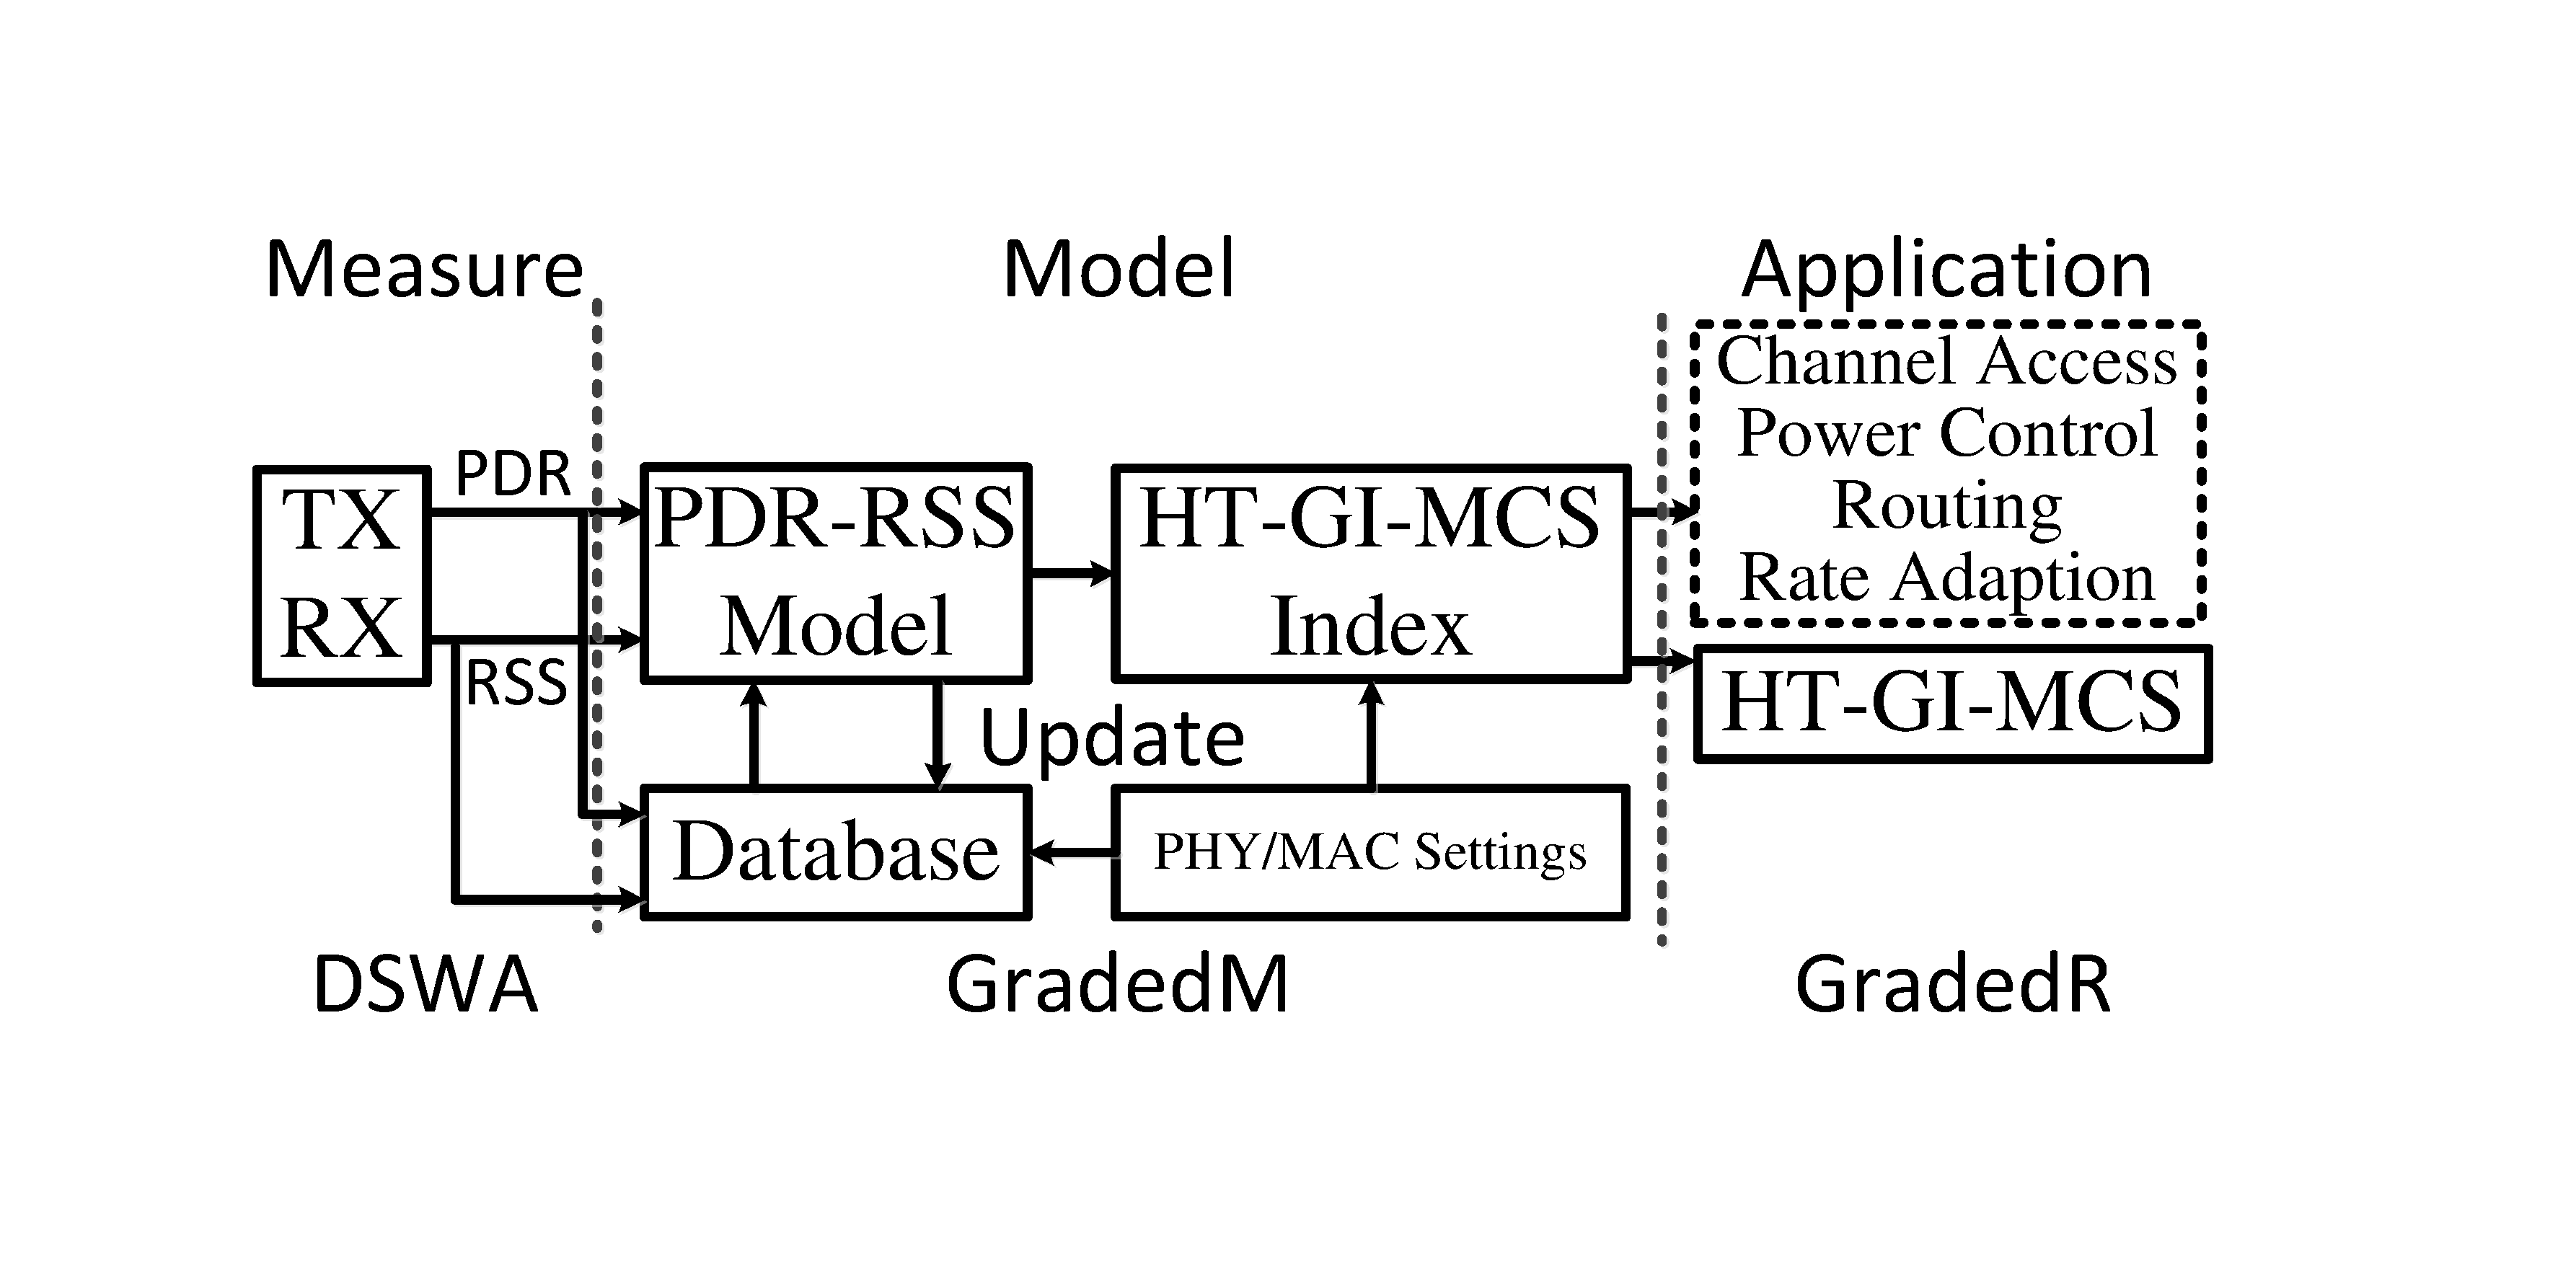
\includegraphics[width=0.6\textwidth]{modeling.pdf}
\caption{Online PDR-RSS modeling framework.}
\label{onlinemodel}
\end{figure}

\section{Literature Review}

\subsection{Packet Delivery Modeling}
There are numerous work on practical delivery and interference modeling. Some early researches paid attention to offline models in static wireless networks \cite{kolar2011mesh} \cite{reis2006model}, and it is widely used in upper layer applications such capacity analysis \cite{kashyap2007capacity} and rate control \cite{chen2011ram} \cite{judd2008efficient}. The authors in \cite{10.1109/TMC.2009.87} proposed repeatable measurement in mobile wireless networks that aimed at combining real experiments and simulations. The Sybot in \cite{kim2010sybot} also conducts mobile spectrum survey which only makes RSS measurement but ignore the link level quality. These works are all based on traditional 802.11a/b/g that can not be directly applied in 802.11n networks. A number of studies have investigated the experimental features of 802.11n networks recently \cite{Halperin2010predictable} \cite{k.rayanchu:fluid:}. The authors in \cite{Halperin2010predictable} provided accurate delivery prediction for MIMO-OFDM of 802.11n based on CSI. But the channel estimation of CSI \cite{CSI-SF} requires too much PYH/MAC operations which makes it more complicated for online measurement and modeling.

\subsection{Rate Adaption}
There are extensively large number of approaches on 802.11n rate control based on simulations or experiments \cite{kim2009experimental} \cite{Pefkianakis:2010} \cite{zhang2008practical}. Some works have been deployed default on Linux platforms, for instance Minstrel \cite{minstrel} for \texttt{mac80211} and Atheros for \texttt{ath9k} \cite{wong2008wireless}. However, these works are designed for static 802.11 networks, which utilize fixed EWMA calculations to process PDR and spend look around frames to detect available data rates. Some approaches were proposed on rate adaption in mobile environments, but most of them are concentrated on RSS measurement \cite{chen2011ram} \cite{judd2008efficient}.

Some upper layer applications such as intrusion detection \cite{5620919} and congestion control \cite{floyd2000equation} employ online PDR measurement methods, but the above proposals do not focus on PDR-RSS modeling and rate selection related issues. To address the mobility and dynamic requirements, our study adopts dynamic sliding window average to measure and predict current PDR values adaptive to environmental changes, and get the most suitable data rate according to online PDR-RSS modeling.

\section{Statement of Significance}
We answer the first question by proposing a Dynamic Sliding Window Average (DSWA) algorithm. DSWA requires only parts of history results to emphasize on the most recent status. In order to deal with the mobility and dynamic requirements, the statistical intervals are event-driven that are determined by the weighted average of previous PDR results. Then the PDR-RSS models can be constructed based on a database, which includes all the raw data from empirical experiments. At the end, we present the GradedM to select the optional configurations based on distance criterion, which outputs the diversity configurations with high reliability performance.

To demonstrate the advantage of online PDR-RSS modeling framework further, we develop a rate adaption algorithm, Graded Rate or GradedR, which adopts an online rate selection process with high precision. Through a real world implementation on our testbed, we evaluate the GradedR over different scenarios and routes. The experimental results indicate that GradedR can achieve throughput gains up to 40\% over the Minstrel rate control algorithm under different MIMO configurations.

In summary, the key contribution of this work is to develop an online PDR-RSS modeling framework, which provides a system-level solution scheme for channel measurement and prediction in Mobile 802.11n networks. The distinctive characteristics of proposed online framework are summarized below:
\begin{enumerate}
\item
\textbf{Accurate PDR measurement in fast changing channels.} Compared with the traditional Exponentially Weighted Moving Average (EWMA) method, DSWA can improve the measurement accuracy by 89\% in mobile scenarios.
\item
\textbf{Dynamic model with low-overhead modeling initialization.}  The PDR-RSS model is updated with real-time PDR and RSS, which initialization requires only \textit{O}$(w\cdot r\cdot g)$ empirical trials as opposed to CSI approaches of \textit{O}$(k\cdot m\cdot n)$, where $w$, $r$, and $g$ denote possible channel widths, PHY data rates and GI lengths respectively.
\item
\textbf{Diversity configurations output with high reliability performance guaranteeing.} GradedM selects the optional configurations from online PDR-RSS model based on current network conditions. Thus, online PDR-RSS modeling framework overcomes the channel quality capturing problem in static PDR-RSS models.
\end{enumerate}


\section{Research Methodology}

\subsection{Packet Delivery Measurement} \label{sect:methodology}

In the traditional rate control algorithms of Atheros's Linux wireless drivers, both \texttt{Madwifi} for 802.11a/b/g and \texttt{ath9k} \cite{ath9k} for 802.11n, EWMA is used to process PDR of each configuration, as shown in Fig.~\ref{weighted}. EWMA has some deficiencies when applied in mobile 802.11n. First, the setting of weighting coefficient $\alpha$ is difficult to respond promptly to link quality changes \cite{EWMAChart}, and it is set fixed to 0.125 or 0.25 in practical implementation \cite{ath9k} \cite{minstrel}. The update cycle is also fixed to 50ms or 100ms, which can not achieve effective control on accuracy and overhead. This will lead to PDR overestimation at high data rates as shown in Fig.2a.

\begin{figure}[!t]
\centerline{
\subfloat[EWMA, weighted window]{
    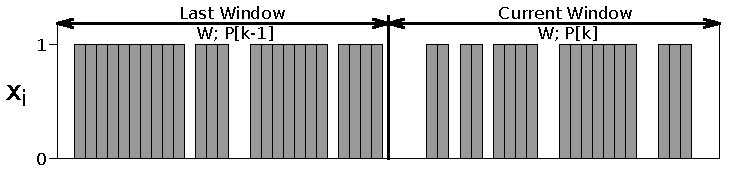
\includegraphics[width=0.5\textwidth]{m_weighted.pdf}
    \label{weighted}
}
%}
%\centerline{
\subfloat[DSWA, sliding window]{
    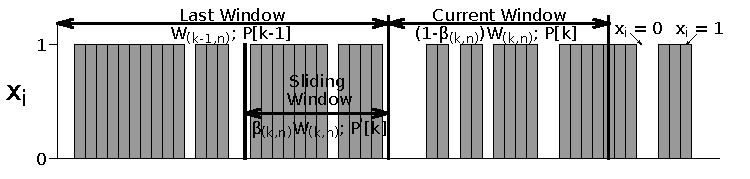
\includegraphics[width=0.5\textwidth]{m_sliding.pdf}
    \label{sliding}
}
}
\caption{Averaging window length in PDR measurement}
\label{method}
\end{figure}

To evaluate the performance of different measurement methodologies, the received status of each transmitted packet $i(i=1,2,3...)$ is defined as a discrete-time stochastic process that only canonically takes 0 and 1. It can be simplified to $x_i=\{0,1\}$, where $x_i=1$ denotes that the $i$-th packet is received successfully. The probability of $x_i=1$ i.e. $\textbf{P(}x_i=1\textbf{)}=p_i$ can be expressed by the standard SINR model or measurement-based PDR-RSS model as follows:
\begin{equation}
 p_i=\textbf{P(}SINR_i(t)>\delta\textbf{)}=\textbf{P(}\frac{R_i(t)}{I_i(t)+n}>\delta\textbf{)}=\hat{p}(R_i(t))
\label{p_i}
\end{equation}
where $SINR_i(t)$ is the packet level SINR of the $i$-th packet transmitted at the time of $t$, $\delta$ is the SINR threshold, $R_i(t)$ is the RSS at time of $t$, $I_i(t)$ is the interference which is composed of all undesirable signals $R_j(t)$ that arrive at the receiver, and $n$ is the thermal noise floor which is usually assumed constant. $\hat{p}(R_i(t))$ is the packet delivery function based on realistic measurement, which is in relationship with the measured RSS. 

For the statistical PDR-RSS model based on realistic measurement in mobile wireless networks, there is a trade-off between measurement accuracy and overhead. The measurement period should be set short enough and responding rapidly to changing network status, or be long cycle to reduce overhead when link quality is steady and reliable. At the same time, both RSS and PDR have time varying and location difference features in mobile 802.11n. And the diversification in data rates and packet size will significantly complicate the programming process. We propose DSWA approach attempting to resolve this dilemma. The measured PDR can be calculated by
\begin{equation}
 \hat{P_s}[k]=\beta P'[k]+(1-\beta)P[k]
 \label{P_s}
\end{equation}
where $\beta=\frac{T}{W}$ is defined as the sliding factor, and $T$ and $W$ are the length of sliding window and the current averaging window. As is shown in Fig.~\ref{sliding}, $P'[k]$ and $P[k]$ respectively denotes the PDR value of sliding and current window.

The parameter settings of $W$ and $\beta$ have significant impact on measurement accuracy and overhead. The average interval $\overline{W}_{(k,n)}$ and sliding factor $\overline{\beta}_{(k,n)}$ for $k$th compute cycle are calculated as follows:
\begin{equation}
  \overline{W}_{(k,n)} = \frac{\sum_{i=1}^n{\omega_i \gamma_i} \eta_{i}}{\sum_{i=1}^n{\omega_i}}
\label{W_s}
\end{equation}
\begin{equation}
  \overline{\beta}_{(k,n)} = 1 + \frac{\sum_{i=1}^n{\omega_i \gamma_i}}{\sum_{i=1}^n{\omega_i}}
\label{beta}
\end{equation}
where $\omega_i$ is the average weight that
\begin{equation}
  \omega_i = \frac{1}{2^{\lfloor\frac{n-i}{2}\rfloor}},~1\leq i \leq n,
\end{equation}
$\gamma_i$ is the factor of relative PDR changes that
\begin{equation}
  \gamma_i = 1 + P[k-n+i] - P[k-n+i-1],~~ 1 \leq i \leq n,
\label{gamma_i}
\end{equation}
and $W_i$ is the window length of last $n$ sequences that $\eta_i=W_{(k-n+i,n)}$. In practice, a value of $n=8$ gives the weights $\omega_i=\{1/8,1/8,1/4,1/4,1/2,1/2,1,1\}$ to emphasize on the most recent status, which can achieve steady and sensitivity responding to different network conditions. Unlike EWMA, the window length $W$ is event driven and unrelated to data rates, and DSWA takes advantage of sliding window averaging to emphasize on the most recent status. Since $\omega_i$ and $\gamma_i$ are associated with the relative changes of PDR, DSWA will make adjustment to $W$ and $\beta$ according to current status. The measurement errors expectation of DSWA can be calculated by:
\begin{equation}
\begin{split}
 \textbf{E[}\Delta P_s[k]\textbf{]}&=\textbf{E[}\beta P'[k]+(1-\beta)P[k]-p_{n}\textbf{]}\\
                                       &=\beta\textbf{E[}P'[k]\textbf{]}+(1-\beta)\textbf{E[}P[k]\textbf{]}-p_{n}\\
                                       &=\beta\overline{p'}[k]+(1-\beta)\overline{p}[k]-p_{n}
\end{split}
\label{Eps}
\end{equation}
where $\overline{p}[k]$ and $\overline{p'}[k]$ are respectively the estimation of $P[k]$ and $P'[k]$, which can be derived from Equation (\ref{P_s}) that $\textbf{E[}P[\cdot]\textbf{]}=\frac{1}{N}\sum\textbf{E[}x_i\textbf{]}=\frac{1}{N}\sum{p_i}=\overline{p}[\cdot]$, where $N$ is the window length, and $\overline{p}[\cdot]$ is the expectation of $p_i$ during the average interval. And $p_n$ is the received probability of last packet which can be deemed as the true PDR value. It can be inferred from Equation (\ref{Eps}) that the measurement errors are associated with $p_i$ changes, which have different features in static or mobile wireless networks. Assuming the same average intervals, it will increase the measurement errors when $p_i$ encounters with sudden changes in short time scale. The detailed experimental evaluation will be given in Section \ref{experiment}.

For the PDR measurement in static wireless networks, the signal strength is approximately fixed for stationary nodes \cite{reis2006model} and then $p_i$ can be deemed as constant during the averaging process. Since then, $x_i$ is independent and identically distributed random variables, which can be characterized by a Bernoulli process that $\textbf{P(}x_i=1\textbf{)}=p$. When $p_i$ are approximately constant for stationary nodes, both methods can get unbiased estimation of $p_i$. For $p_i=0.8+\sigma$ where $\sigma\sim \textrm{N}(0,0.01)$ is ambient noise, the measured results, whose mean values are 80.23\% and 80.06\% respectively, are both close to the true value of $p_i=0.8$. But DSWA can achieve lower overhead in this case, which will be explained later.

However, in the measurement of realistic networks, EWMA can hardly get sufficient measurement accuracy compared to DSWA. In mobile wireless networks, the propagation environments are complex and communication terminals are on the move particularly, which means the RSS and interference are changing during PDR measurement. This will make the packets received probability $p_i$ changes in short time scale. In this case, it can be characterized by a Generalized Bernoulli process that the probability of $x_i=1$ is different for all values of $i$.

Fig.~\ref{cdf} illustrates the CDF of measurement errors for EWMA and DSWA when applied in mobile scenarios. The measurement errors are within $\pm$0.008 for DSWA, and change from -0.019 to 0.032 for EWMA. The errors of EWMA show that it tends to overestimate the actual PDR, which can also be seen from Fig.~\ref{cdf} that the overall CDF curve of EWMA errors shift to the right of line $Error=0$. Compared with the traditional EWMA method, DSWA can improve the overall measurement accuracy of 89\% higher in mobile scenarios.
\begin{figure}[!t]
\centerline{
    \subfloat[CDF of errors]{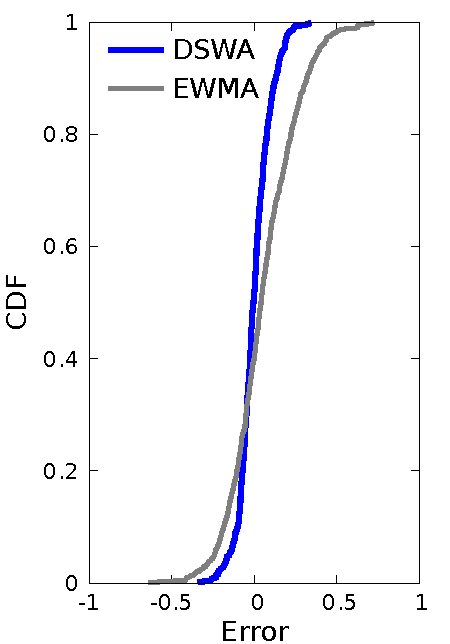
\includegraphics[width=0.3\textwidth]{cdf.pdf}
\label{cdf}
}
\subfloat[Window length and sliding factor of DSWA]{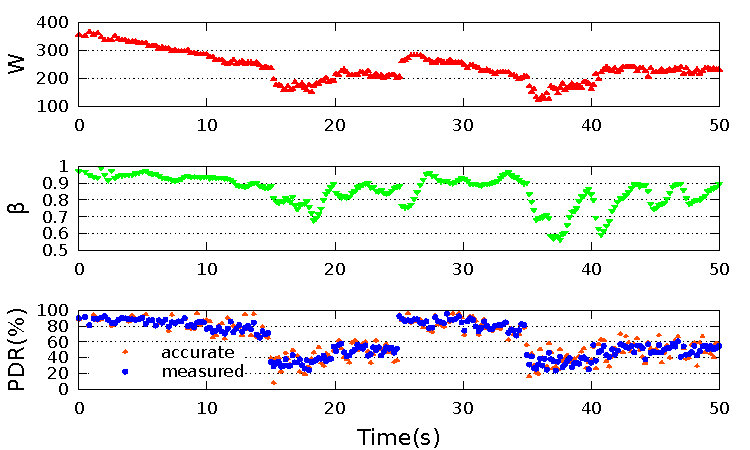
\includegraphics[width=0.7\textwidth]{DSWA.pdf}
\label{overhead}
}
}
\caption{Measurement results of EWMA and DSWA in mobile scenarios.}
\label{DSWA_error}
\end{figure}

In addition to meet the accuracy requirements, it also deserves attention to reduce measurement overhead, since more sample packets will lower the throughput achieved. The sampling intervals of DSWA are weighted average of last $n$ results so that it can reduce mutations caused by noise and respond quickly to real changes of PDR values. Moreover, the averaging intervals of DSWA are associated with PDR changes to allow a more timely response to sustained decreasing in link quality, and make less frequent samples as network conditions are in steady continuously. Fig.~\ref{overhead} shows an example of DSWA for measuring PDR adaptive to different network conditions. The packet delivery has a sudden decrease at the time of about 15s, and both average interval $W$ and sliding factor $\beta$ drop accordingly. When PDR increases and getting stable from 40s to 50s, $W$ changes from 100 to 200 which will reduce measurement overhead significantly. The average window length of EWMA are approximately constant for certain rate that $W=20$ for 6.5Mbps and $W=500$ for 300Mbps. EWMA can not respond timely when $W=500$ and result in unnecessary errors, especially when there is sudden PDR decline.

\subsection{Channel State Estimation} \label{sect:estimation}
To reduce the computing complexity and overhead of channel state estimation,

\subsection{Packet Delivery Modeling} \label{sect:modeling}
Based on the insights from Section \ref{motivation}, we propose an online PDR-RSS modeling framework in Fig.~\ref{onlinemodel}. This framework is composed of three main components: Database, PDR-RSS model, and HT-GI-MCS index. The database contains the raw data of PDR and RSS along with different 802.11n PHY/MAC settings. The PDR-RSS model is a set of data pair for transition windows' lower and upper bound. HT-GI-MCS index is the configuration selection sequence. The construction of the online framework is consist of the following three steps. First, the database is initialized through empirical experiments. Then it will be updated to the PDR-RSS model under different settings in realtime operating. Finally, the HT/GI/MCS selection sequence can be generated according to the online PDR-RSS model and current status, which can provide optional HT/GI/MCS in order that can provide reliable communications (PDR$>$90\%).

Compared to the general static PDR-RSS modeling framework in Fig.~\ref{offlinemodel}, the proposed online framework has the following distinctive features. First, it has two inputs into both PDR-RSS model and database. Second, both PDR-RSS model and database are updated online. Third, it exploits both real-time PDR and RSS, along with the diversity property to derive the set of configuration(s) with certain reliable performance guaranteeing. Through the distinctive features, the online PDR-RSS modeling framework can provide a systematic solution for the channel quality capturing problem in static PDR-RSS models. In the following, we give a thorough design process for the online framework to demonstrate how to address the three critical issues: high-accuracy PDR measure, dynamic PDR-RSS model update and efficient configuration output, in online framework.

\begin{figure}[!t]
\centerline{
    \subfloat[GI = 400ns]{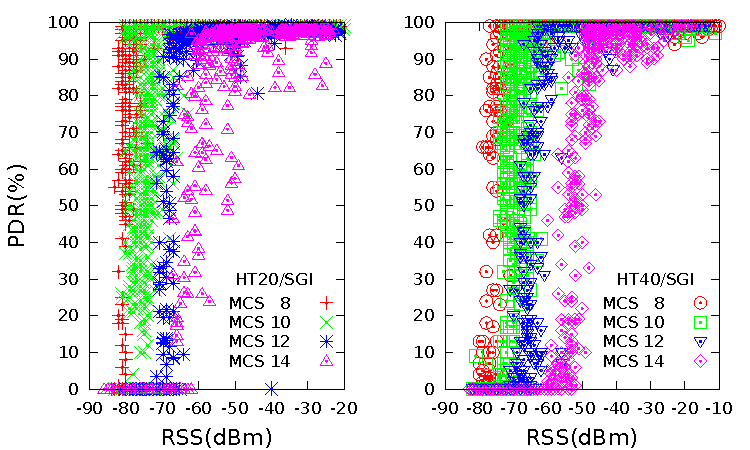
\includegraphics[width=0.45\textwidth]{pdr_ch_sgi.pdf}
    \label{pdr_sgi}
}
    \subfloat[GI = 800ns]{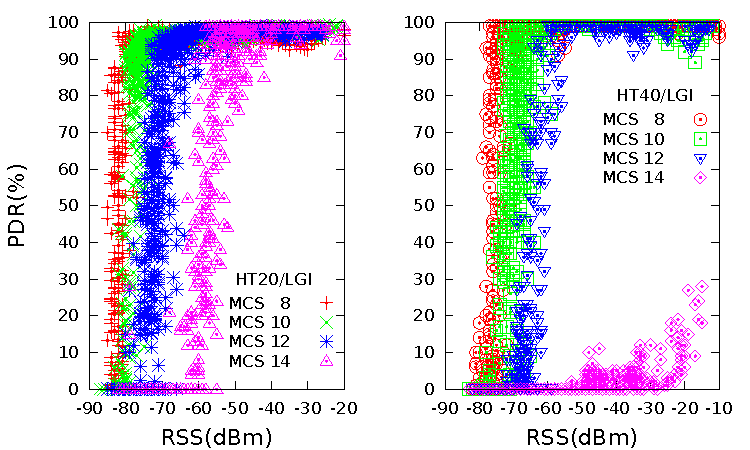
\includegraphics[width=0.45\textwidth]{pdr_ch_lgi.pdf}
    \label{pdr_lgi}
%}
%    \subfloat[MCS 15]{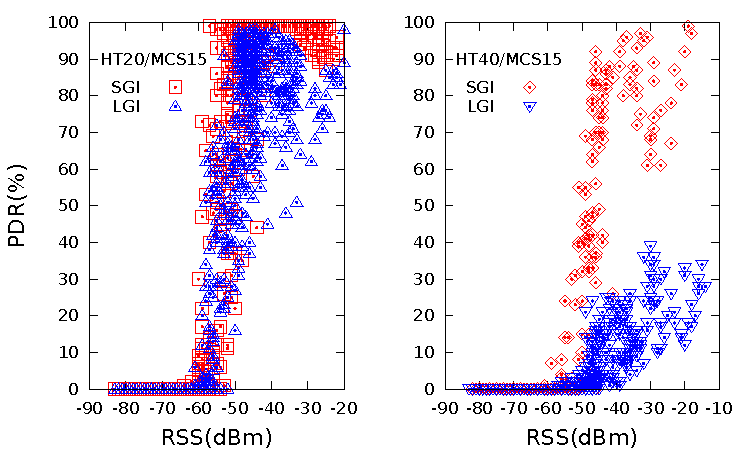
\includegraphics[width=0.33\textwidth]{pdr_sgi.pdf}
%    \label{pdr_sgi_high}
}
}
\caption{PDR-RSS model under different channel types and data rates.}
\label{pdr}
\end{figure}

The 802.11n standard incorporates PHY/MAC enhancements to achieve higher throughput and wider coverage. In the PHY layer, 802.11n networks adopts MIMO technology to achieve spatial multiplexing and diversity. 802.11n utilizes channel bonding technology, with which two adjacent 20MHz channel is united to a new 40MHz one, to realize higher data rates. In the MAC layer, 802.11n also employs SGI and frame aggregation to reduce overhead and improve efficiency. All these PHY and MAC enhancements not only play an effective impact on the performance of higher layers, but also make link quality measurement and analysis more complicated. For above configurations of 802.11n, the PDR-RSS model shows different characteristics.

To construct the database and PDR-RSS model in the online framework, we conduct extensive experiments to illustrate the relationship between PDR-RSS model and 802.11n PHY/MAC amendments, including data rates, channel widths and GI lengths. For all MCS indexes of 0-23, channel widths of HT20/HT40, GI lengths of LGI/SGI, 6 moving routes and 11 locations, the above experiments contains at least 500 trials to cover most of 802.11n network status. The following is the summary of experimental results.

\begin{enumerate}
  \item \textbf{Data Rates:} We first illustrate the influence of different PHY data rates on PDR, and both HT20/HT40 and LGI/SGI cases are investigated. Fig.~\ref{pdr} presents the measured PDR-RSS function under different data rates. First, the receiver sensitivity gets higher with the increase of data rates, that from -80dBm to -50dBm of HT20/SGI and -80dBm to -40dBm of HT40/SGI when the MCS changes from 8 to 14. Second, the transition window length $\rho$ also increases along with data rates, especially as the data rates are higher than 115Mbps. As can be seen in Fig.~\ref{pdr_sgi} that $\rho$ can even achieve 15dB when the MCS rate index is 12, which will significantly reduce 802.11n networks' efficient throughput.
  \item \textbf{Channel Widths:} 802.11n defines the use of 20MHz and 40MHz channels, and 40MHz channels allow data rates up to 150Mbps for each spatial stream. It provides more than double the data rates 20MHz channels when link quality is good. However, 40MHz channels are more sensitive to even small interference. As can be seen in Fig.~\ref{pdr_sgi}, the receiver sensitivity of 40MHz channels are higher for both LGI and SGI under different PHY data rates. The transition windows lengths are almost the same for both 20MHz and 40MHz channels, which vary from 3dB of MCS 8 to 10dB of MCS 14. It is also observed that 40MHz has an unexpected benefit of range improvement at moderate data rates, that it can provide the same data rate at a more wider coverage.
  \item \textbf{Guard Interval:} To increase data rate, 802.11n added optional support for a 400ns SGI, which can provide an 11\% increase of data rate in theory \cite{perahia2008next}. There is little difference in PDR and throughput when data rates are low, which is presented in Fig.~\ref{pdr}. But when data rates get higher, SGI can improve network performance obviously, especially for HT40 channels. One case is given in Fig.~\ref{pdr_sgi_high} that the PDR values are never higher than 40\% for MCS15 of HT40/LGI. The measurement results show that SGI can respectively achieve 10\%-40\% and 20\%-60\% higher PDR for HT20 and HT40 channels.
\end{enumerate}

\begin{figure}[!t]
\centering
    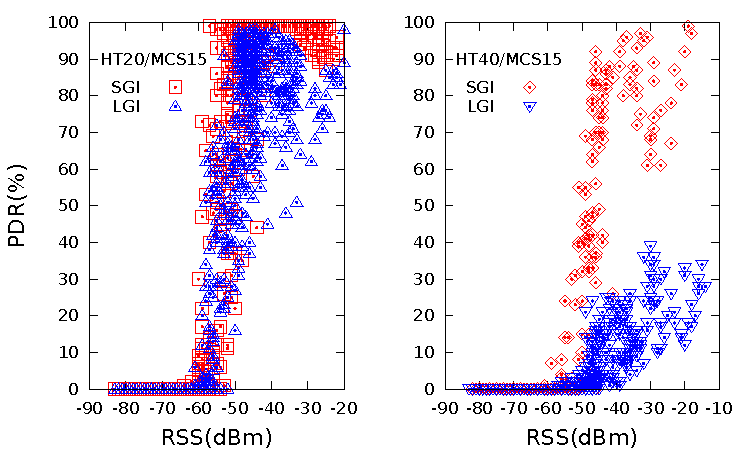
\includegraphics[width=0.5\textwidth]{pdr_sgi.pdf}
\caption{The influence of SGI on PDR-RSS model at high data rates.}
\label{pdr_sgi_high}
\end{figure}

\subsection{Upper Layer Requirements} \label{sect:upper}

\begin{enumerate}
  \item \textbf{Traffic Loads:}
  \item \textbf{Traffic Patterns:}
\end{enumerate}

Through the above characterization, we can initialize the database of online framework. Then a table for the PDR-RSS model can be generalized, which contains the two boundaries of transition windows. We define it as a struct in Linux C code of GradedT for the practical implementation. The initial values of GradedT can be obtained by $\textit{O}(N \cdot w \cdot g \cdot r)$ trials, where $N$ is the number of stationary nodes or mobile routes, $w$ is the channel widths with certain center frequencies, $g$ is the GI length and $r$ is the MCS indexes. For 802.11n networks with 3x3 MIMO, $w=2$ for HT20/HT40 at 5GHz frequency, $g=2$ for LGI/SGI, $r=24$ for MCS 0-23.

An example of GradedT of 2x2 MIMO has been given previously in Fig.~\ref{MCS} (Section \ref{motivation}), and this table is updated in real-time operating. GradedT separates the HT/GI/MCS selection and RSS into three regions that locating just the right of gray line will efficiently improve achieved throughput with high reliability. In Section \ref{motivation}, we have stated the diversity property of transition windows for different configurations in 2x2 MIMO. The same observation can be derived from GradedT of 3x3 MIMO. Due to page limitation, we omit the detail experimental results in this paper.
\subsection{Online PDR-RSS Modeling}
The online PDR-RSS modeling is to update the PDR-RSS model and database, and generate the HT/GI/MCS selection sequence according to current network conditions. We name this online modeling process as GradedM. Obviously, we can identify the reliability by the distance between transition windows' upper bound and current RSS. Then GradedT is sorted in order by the distance, and the HT/GI/MCS selection sequence is generated accordingly. The pseudo code of GradedM is shown in Procedure \ref{alg_graded}.
\begin{algorithm}[!t]
\floatname{algorithm}{Procedure}
\renewcommand{\algorithmicrequire}{\textbf{Input:}}
\renewcommand{\algorithmicensure}{\textbf{Output:}}
\caption{GradedM: online PDR-RSS modeling}
\label{alg_graded}
\begin{algorithmic}[1]
\Require pdr-now,rss-now
\Ensure  ht-gi-mcs-index
\State{\label{graded-table}struct GradedT \{ \\ ~~~~~graded-delta[r][2]; // r=8/16/24 for 1/2/3 spatial streams\\ \} graded-table[w][g]; // w=g=2 for HT20/HT40 LGI/SGI\label{graded-table2}}
\If{graded-delta-changed} \label{delta-changed}
\State{graded-table $\gets$ update-delta(pdr-now,rss-now);}
\EndIf \label{delta-updated}
\State{mcs-index $\gets$ sort(graded-table,rss-now);} \label{ht-gi}
\State{ht-gi-mcs-index $\gets$ sort(mcs-index,mcs-rate);} \label{ht-gi-mcs}
\State \Return{ht-gi-mcs-index;}
\end{algorithmic}
\end{algorithm}

The struct GradedT (line \ref{graded-table} to \ref{graded-table2}) defines the upper and lower limits of transition windows for different HT/GI/MCS. When the limits are changed, which can be determined by current PDR and RSS, the table will be updated (line \ref{delta-changed} to \ref{delta-updated}). For all the HT/GI/MCS options that locate on the right of the gray line, GradedM will first sort GradedT into HT/GI selection sequences (line \ref{ht-gi}) by the distance (in dB value) of current RSS and every transition windows\rq upper bound. Then the HT/GI/MCS index (line \ref{ht-gi-mcs}) can be generated according to the available data rates that each HT/GI/MCS option can provide. Noting the configurations generated in GradedM provide different combinations of data rate and reliability, which enables diversity choice for the upper layer applications.

The complexity of the online PDR-RSS modeling framework is mainly composed of measurement, construct and update of database and PDR-RSS model, and GradedM algorithm. In the measurement phase, DSWA is unrelated to configurations. For the initialization of data base, it requires at most \textit{O}$(w\cdot g \cdot r)$ trials, and GradedM's computational complexity is at most \textit{O}$(r \log{r})$. Since the available $r$ that will be sorted is far less than the maximum MCS index, the overall complexity of online PDR-RSS modeling is \textit{O}$(w\cdot g \cdot r)$.


\subsection{Rate Adaption Algorithm}

\begin{figure}[!t]
\centering
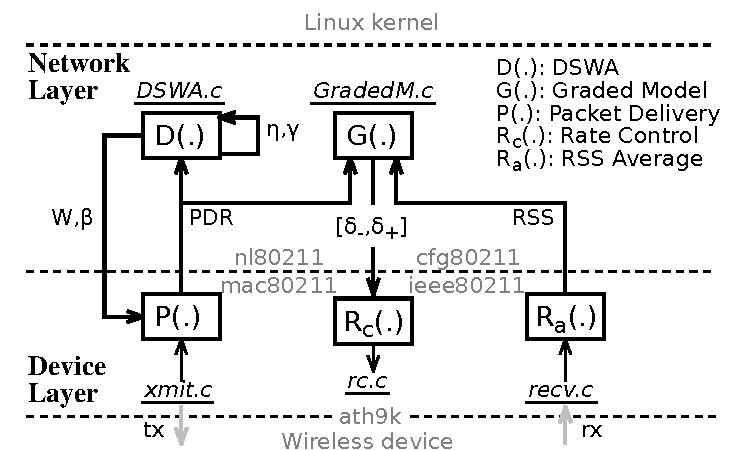
\includegraphics[width=0.8\textwidth]{framework.pdf}
\caption{Measurement framework and implementation on Linux systems.}
\label{framework}
\end{figure}

GradedR adopts DSWA to get accurate PDR measurement with low overhead, then chooses the suitable configuration according to HT/GI/MCS index. The pseudo code of above process is shown in Procedure \ref{alg_pdr}, and the PDR threshold in GradedM.c is set to \{$P_{thrl},P_{thrh}$\}=\{$10\%,90\%$\}. When the selected MCS is far away the right bound of its transition window, GradedR will choose a new configuration to acquire a higher data rate. On the contrast, it will reduce the data rate when current PDR falls into the transition window. Given the characterization results in Section \ref{modeling}, we only select SGI as the final rate adaptation step when the link quality is still poor running at the highest rates of LGI.
\begin{algorithm}[!t]
\floatname{algorithm}{Procedure}
\renewcommand{\algorithmicrequire}{\textbf{Input:}}
\renewcommand{\algorithmicensure}{\textbf{Output:}}
\caption{GradedM $\rightarrow$ DSWA $\rightarrow$ GradedR}
\label{alg_pdr}
\begin{algorithmic}[1]
\Require tx-complete (packets transmitted event)
\Ensure  rate-index (rate selection indexes of HT/GI/MCS)
\State{// DSWA(pdr-last,pdr-now): return averaging window length $W$ and sliding factor $\beta$, update $\gamma$ and $\eta$}
\State{// GradedM(pdr,rss): update the graded-table and sort it into MCS selection sequences, return ht-gi-mcs-index}
\State{// GradedR(ht-gi-mcs-index): return ht-gi-mcs, ensure current PDR out of the transition window with the highest available data rate}
\If{pdr-now $<P_{thrh} |$ rss-now $<\delta_+$}
\State{graded-talbe $\gets$ GradedM(pdr-now,rss-now);} // rc.c
\State{rate-index $\gets$ down-rate-mcs(ht-gi-mcs-table);}
\EndIf
\If{graded-sens - rss-now $>$ high-limit-to-gray}
\State{rate-index $\gets$ up-rate-mcs(ht-gi-mcs-table);}
\EndIf
\State \Return{\{tx-status,rate-index\};}
\end{algorithmic}
\end{algorithm}

We implemented above algorithm on Linux systems with modified \texttt{ath9k} wireless driver. Fig.~\ref{framework} illustrates the software architecture, which is composed of both network layer and device layer components. The network layer conducts DSWA calculations to determine averaging intervals and sliding factor, and makes GradedT update to get rate selection indexes. On the device layer, it is driven by transmitting and receiving events that execute PDR computation and RSS averaging respectively. The rate indexes are also selected on device layer according to results of network layer when the PDR or RSS is lower than transmission threshold.


%\nocite{*}

\renewcommand\refname{References}
%\bibliographystyle{alpha}
\bibliographystyle{apalike}
%\IEEEtriggeratref{6}
\bibliography{wireless}
%\printbibliography

\end{document}
